Radioactivity has been present in the Universe since its inception. It was an important element of the Big Bang\footnote{The Big Bang is the most acceptable hypothesis that explains the formation of the universe and its development over time so far.}, which occurred about $14 \cdot{} 10^9$ years ago. It was also present during the formation of the earth, $4.5 \cdot{} 10^9$ years ago, which explains why the different layers that make up the earth contain radioactive elements. 

Therefore, humanity has been exposed to radioactivity since its origin, whether present in the Earth's crust or in the universe (external natural irradiation). Even the human being himself is radioactive as radioactive elements are contained in the human body such us $\ce{^{3}H}$, $\ce{^{14}C}$ or $\ce{^{40}K}$, introduced into the body through food or water ingestion or air inhalation (internal natural irradiation). The annual average of the radioactive dose received by the population is presented in Figure \ref{fig:RadioactiveDosePopulation} and Table \ref{tab:RadioactiveNaturalDosePopulation}.

\begin{figure}[h]
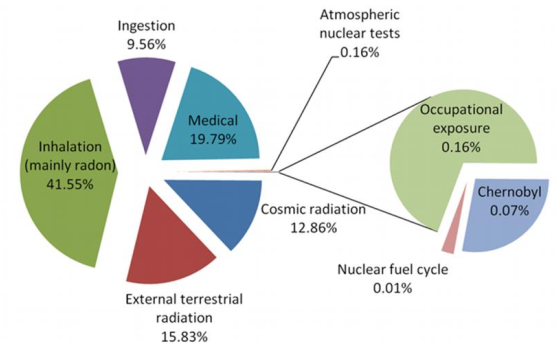
\includegraphics[scale=0.5]{2Introduction/RadioactiveDosePopulation.png}
\centering
\caption{Annual average distribution of the radioactive dose received by the population~\cite{IAEA}\label{fig:RadioactiveDosePopulation}}.
\end{figure}


\begin{table}[htbp]
\begin{center}
\begin{tabular}{|c|c|c|}
\hline
Radiation source & Eff. dose ($\milli\sievert/$yr) & Typical range ($\milli\sievert/$yr)\\
\hline \hline \hline
Cosmic (external) & $0.39$ & $0.3 - 1.0$ \\ \hline
terrestrial (external) & $0.48$ & $0.3-0.6$ \\ \hline
\hline  
Inhalation (internal) & $1.26$ & $0.2-10$ \\ \hline
Ingestion(internal) & $0.29$ & $0.2-0.8$ \\ \hline
\hline 
Total & $2.42$ & $1-12.4$ \\ \hline
\end{tabular}
\caption{Annual average distribution of the effective dose received by the population due to natural radioactive~\cite{UNSCEAR, CSN}.}
\label{tab:RadioactiveNaturalDosePopulation}
\end{center}
\end{table}

As can be seen in Figure \ref{fig:RadioactiveDosePopulation}, most of the radioactive dose received by the population is due to both, internal and external natural radiation, called natural radiation, the effective dose\footnote{The effective dose is the radioactive dose absorbed by the population, taking into account the different radiosensitivity in each organ or tissue.} of which is estimated in $2.42~\milli\sievert/$yr as can be seen in Table \ref{tab:RadioactiveNaturalDosePopulation}. It can also be appreciated in Figure \ref{fig:RadioactiveDosePopulation} that the most important part of the artificial radiation received comes from medical purposes. 

Since the discovery of radioactivity, made by Hènri Becquerel in $1896$, a lot of technology based on nuclear concepts has been developed and applied to several fields such as energy production, research, medicine, industry, etc. 

Due to the introduction of radioactivity in the society, various anthropogenic radioactive sources have appeared in the environment, resulting in increased levels of its radioactive elements, called radioactive background. 

As our knowledge about radioactivity and our measurement techniques have advanced, the negative effects of radioactivity have been observed and characterized. Because of that, it is important to control the level of radioactive background to which the population is exposed and to ensure that these levels is kept below of a safe limit. For this task, several organizations was created to manage the radioprotection in the world.

\begin{enumerate}
\item{} Firstly, a definition of concepts and units was necessary to quantify the negative effects of radioactivity and, for that, the International Commission of Radiological Units and Measurements, ICRU \cite{ICRU}, was created during the first international conference of radiology held in London, in 1925.

\item{} Secondly, the International Commission on Radiological Protection, ICRP \cite{ICRP}, was created in 1928 by the International Society of Radiology, ISR \cite{ISR}. The ICRP aims to make recommendations and to provide guidance on different aspects of protection against radioactivity. The ICRP does not have the legal capacity to enforce its recommendations, but these are widely taked into account in the legislation of most countries. %is fairly consistent with them.

\item{} Thirdly, the United Nations Scientific Committee on the Effects of Atomic Radiation, UNSCEAR \cite{UNSCEAR}, was created in 1955, the objective of which is to estimate and report the levels and effects of ionizing radiation on the population and the environment. These estimates are taken into account by governments around the world to establish their limits and safety standards.

\item{} Fourthly, the International Atomic Energy Agency, IAEA \cite{IAEA}, was created in 1957, which is though to promote the peaceful use of nuclear energy and to avoid its use for any military purpose such us nuclear weapons. Although it is an independent agency, it must to report to the United Nations, UN \cite{UN}.

\item{} Fifthly, at the level of the European Union, EU, the European Atomic Energy Community, EURATOM, was created in 1957, which is a international organization stablished by the EURATOM treaty. Its objective is to coordinate research programs for the peaceful use of nuclear energy and the sharing of knowledge, infrastructure and financing of nuclear energy.

\item{} Finally, at the national level in Spain, the Nuclear Safety Council, CSN for its acronym in Spanish, was created in 1980 \cite{CSN}. The CNS is the only institution in Spain with legal power to manage everything related to nuclear safety and radiological protection and its objective is to reduce to the maximum the radioactivity in the environment due to anthropological origins.

For this task, the CSN has created several networks consisting of several detectors of radioactivity that are in charge of controlling the levels of radioactivity in the environment and checking the impact of radioactivity facilities to it. Two of the most important networks are the network of automatic stations and network of sampling stations:

\begin{enumerate}
\item{} On the one hand, the network of automatic stations \cite{REA}, REA for its acronym in Spanish, shown in Figure \ref{fig:REA}, which consists of several gamma detectors\footnote{Detectors that only measure gamma radioactivity} distributed in Spain that measure the radioactive dose in real time. The REA is used for the immediate detection of radiological problems and the application of quick response.

\item{} On the other hand, the network of sampling stations \cite{REM}, REM for its acronym in Spanish, shown in Figure \ref{fig:REM}, which consists of several interesting points in Spain where samples are taken and transported to a laboratory to be measured. About twenty Spanish laboratories are integrated into this network, the objective of which is to characterize the concentration and evolution of various radioisotopes present in the radioactive background of Spain and to quantify the impact of radioactive facilities on the environment.
\end{enumerate}

\begin{figure}[hbtp]
 \centering
  \subfloat[Measured points of the REA \cite{REA}. The white box is the daily average of the gamma dose and the green box is the monthly average of the gamma dose.]{
   \label{fig:REA}
    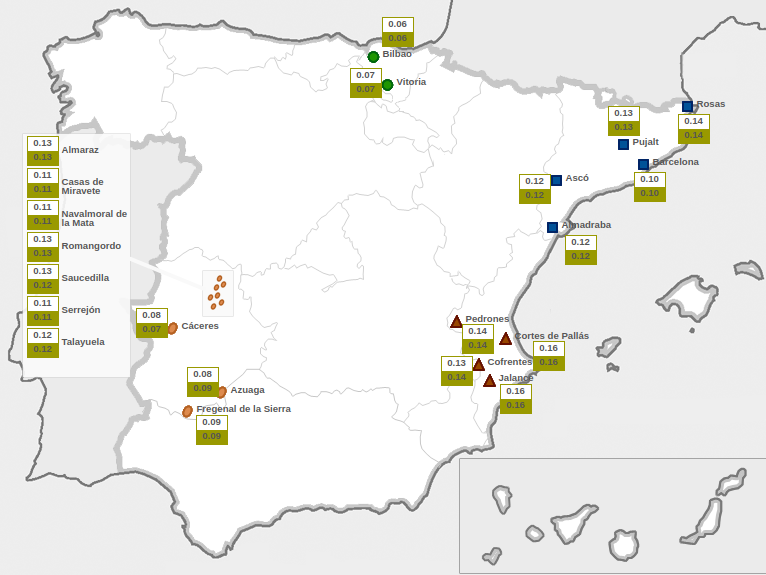
\includegraphics[width=0.5\textwidth]{2Introduction/REA.png}}
  \subfloat[Measured points of the REM \cite{REM}. Blue dots are located around nuclear facilities. Green dots are uniformly distributed in Spain.]{
   \label{fig:REM}
    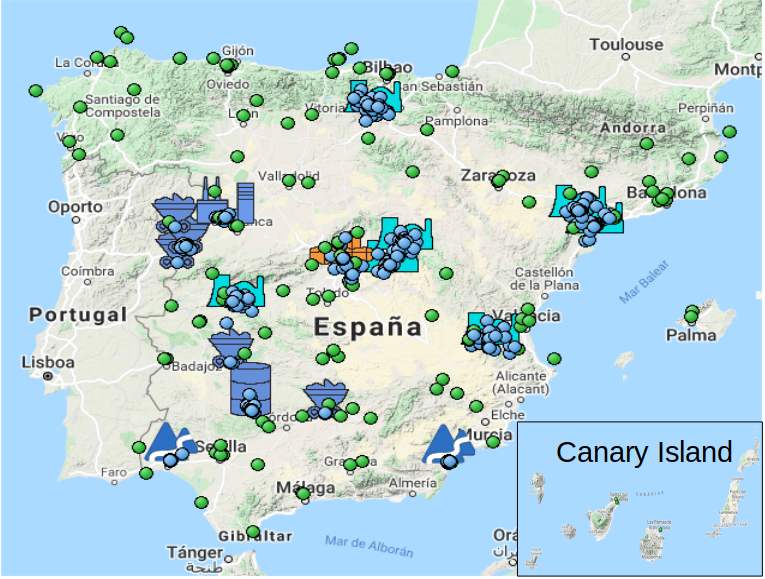
\includegraphics[width=0.5\textwidth]{2Introduction/REM.png}}
 \caption{Networks of automatic station and sampling station belonging of CSN of Spain.}
 \label{fig:NetworksCSN}
\end{figure}

There are other networks that measure different parameters such as the concentration of $\ce{^{226}Ra}$ in the air and the measurements of all the networks are adapted to the EUROTAM treaty \cite{100BqL}.
\end{enumerate}

The objective of this thesis and the objective of the \textit{TRITIUM} project is to develop a monitor capable of automatically measuring low levels of tritium in water in quasi-real time\footnote{Quasi-real time is an approximation of real-time measurements. It means a relatively small time, like ten minutes.}. This monitor is destined to be finally included in the REA.

Tritium is one of the radioactive isotopes routinely measured in REM tests. Its detection is based on low-energy beta radiation measurements of the radioactive decay of tritium, mainly through the liquid scintillation counter technique, LSC. Due to the limitations of the curret methods, which will be shown in section \ref{sec:StateOfTheArt}, the objective of the \textit{TRITIUM} project is to build a tritium detector based on scintillating fibers that will be put directly in contact with the sample (water). The photons produced in these scintillating fibers will be read out using photosensors, either photomultiplier tubes (PMTs) or silicon photomultipliers (SiPMs). 

The \textit{TRITIUM} collaboration is a international group consisting of a consortium of 6 different southwestern european institution of 3 different countries: Portugal, France and Spain. The final emplacement of the \textit{TRITIUM} monitor is the Arrocampo dam, Extremadura, Spain, the water of which is used for the cooling system of the Almaraz fission nuclear power plant, hereinafter called nuclear power plant, NPP. This detector will be installed 4 km downstream from the Almaraz Nuclear Power Plant.

The monitor will be used to ensure that the tritium levels of the Arrocampo dam  water are below of the legal limit specified in the EURATOM treaty \cite{100BqL}, which is $100~\becquerel/\liter$. It will be used indirectly to verify the correct operation of the Almaraz NPP, located $4~\kilo\meter$ above the river since a malfunctioning of it will produce a increase of the tritium activity.

Tritium is one of the most abundantly produced radioisotope in a NPP, as it was verified in the United States Department of Energy complex, (U.S. DOE) \cite{FiberDetector1a, FiberDetector1b} and in several research facilities in China \cite{CommonEmissionTritium} and places around them (ground water, surface water and process waste water).

%Generally, a nuclear reactor is characterized by high stability and, therefore, by a constant emission of radioactive isotopes. 
Tritium is normally produced in the water used in the nuclear reactor cooling system or the moderator of some NPPs. It is produced by neutron capture of deuterium, existing in the heavy water ($\ce{D_2 O}$), semi-heavy water ($\ce{H D O}$) or the deuterium created by neutron capture in usual water ($\ce{H_2 O}$). All these processes have a large probability to happen due to the huge neutron flux in the nuclear reactor, of the order of $10^{14} ~\ce{n} \, \cm^{-2} \second^{-1}$ \cite{CrossSeccionNeutrons}. This tritium is finally released partially or totally to the environment with a quantity that depends on the reactor type as it is shown in Table \ref{tab:TritiumEmisionsNPPs}. The most common way that tritium is released to the environment is $\ce{HTO}$ \cite{CommonEmissionTritium}.

\begin{table}[htbp]
%%\centering
\begin{center}
\begin{tabular}{|c|c|c|}
\hline
Reactor type & Gaseous discharge ($\giga\becquerel/$y) & Liquid discharge ($\giga\becquerel/$y) \\
\hline \hline \hline
PWR & $3.70\cdot 10^{3}$ & $2.59\cdot 10^{4}$ \\ \hline
BWR & $1.85\cdot 10^{3}$ & $3.70\cdot 10^{3}$ \\ \hline
HWR & $7.40\cdot 10^{5}$ & $1.85\cdot 10^{5}$ \\ \hline
GCR & $7.40\cdot 10^{3}$ & $1.11\cdot 10^{4}$ \\ \hline
\end{tabular}
\caption{Emission of tritium per year from different types of nuclear reactors. Pressurized Water Reactor (PWR), Boiled Water Reactor (BWR), Heavy Water Reactor (HWR) and Gas-Cooled Reactor (GCR) \cite{CommonEmissionTritium}}.
\label{tab:TritiumEmisionsNPPs}
\end{center}
\end{table} 

NPPs are operational since more than 60 years and, nowadays, they are essential for providing a large part of the electic power that is used in the world (more than 20\% in Spain \cite{PercentageEnergySpain}). Although the Spanish government is projecting to progressively shut down all NPP there are other countries like China \cite{60ReactorsChina} or United States, USA \cite{35MillionsUSA}, which intend to promote their use.

On the one hand, NPPs are an interesting investment since it is one of the cheapest source of energy production. It is stable, as it doesn't depend on  meteorological parameters and it doesn't emit greenhouse gases. Although there are other alternative energy sources which are being developed quickly  (photovoltaic, wind, tidal energy, etc.), even other concepts of energy production and saving (local production, solar roofs, energy efficiency, smart cities, etc.), today they are not developed enough to fully cover the population needs. On the other hand, NPPs still have some problems such as the contamination of fresh water from uranium mining, the nuclear waste produced, the nuclear proliferation or the risk of radioactive contamination from accidents as happened in the past: Chernobyl, Fukushima and Three Mile Island \cite{ThreeMileIsland}.

In any case it is not important if people agree or not with nuclear energy source. The only important thing is that the nuclear energy production in the world is not going to stop in the next decade, in fact, it will increase as the United States Energy Information Administration (U.S. EIA) expects \cite{EIAOutlook}. Therefore the development of  different types of alarm systems is a good investment. Safety is not a negotiable aspect and there must be mechanisms that warn us of any malfunction of a nuclear power plant. 

In addition, it is important to highlight that the developed monitor could be used to verify the correct operation of a nuclear power plant, but it is not our objective. Our much broader objective is to ensure that the levels of tritium in the analyzed water are below the Spanish legal limit. It means that this monitor could be used in many different places with radioactive facilities like the future fusion power plants\footnote{The International Thermonuclear Experimental Reactor, ITER, will need up to several tens of kilograms of tritium to function, which correspond to various $\tera\becquerel$ of tritium.}, nuclear research facilities\footnote{Tritium is one of the main emissions from these sites \cite{FERMILAB}, \cite{BrookHavenNationalLaboratory}.} or tracking the movement of tritium contaminated plumes in ground water \cite{TrackingTritium}. 

%which is normally done by liquid scintillation counter technic (LSC). This technic has a very good detection capability and precision but it has the inconvenient of providing a delayed results of about 1-2 days or even more. Liquid scintillation technique for the tritium measurement will be presented in section \ref{sec:StateOfTheArt}.